% Options for packages loaded elsewhere
\PassOptionsToPackage{unicode}{hyperref}
\PassOptionsToPackage{hyphens}{url}
%
\documentclass[
  12pt,
]{article}
\usepackage{lmodern}
\usepackage{amsmath}
\usepackage{ifxetex,ifluatex}
\ifnum 0\ifxetex 1\fi\ifluatex 1\fi=0 % if pdftex
  \usepackage[T1]{fontenc}
  \usepackage[utf8]{inputenc}
  \usepackage{textcomp} % provide euro and other symbols
  \usepackage{amssymb}
\else % if luatex or xetex
  \usepackage{unicode-math}
  \defaultfontfeatures{Scale=MatchLowercase}
  \defaultfontfeatures[\rmfamily]{Ligatures=TeX,Scale=1}
\fi
% Use upquote if available, for straight quotes in verbatim environments
\IfFileExists{upquote.sty}{\usepackage{upquote}}{}
\IfFileExists{microtype.sty}{% use microtype if available
  \usepackage[]{microtype}
  \UseMicrotypeSet[protrusion]{basicmath} % disable protrusion for tt fonts
}{}
\makeatletter
\@ifundefined{KOMAClassName}{% if non-KOMA class
  \IfFileExists{parskip.sty}{%
    \usepackage{parskip}
  }{% else
    \setlength{\parindent}{0pt}
    \setlength{\parskip}{6pt plus 2pt minus 1pt}}
}{% if KOMA class
  \KOMAoptions{parskip=half}}
\makeatother
\usepackage{xcolor}
\IfFileExists{xurl.sty}{\usepackage{xurl}}{} % add URL line breaks if available
\IfFileExists{bookmark.sty}{\usepackage{bookmark}}{\usepackage{hyperref}}
\hypersetup{
  pdftitle={Using intonation to disambiguate meaning:},
  hidelinks,
  pdfcreator={LaTeX via pandoc}}
\urlstyle{same} % disable monospaced font for URLs
\usepackage[margin=1in]{geometry}
\usepackage{graphicx}
\makeatletter
\def\maxwidth{\ifdim\Gin@nat@width>\linewidth\linewidth\else\Gin@nat@width\fi}
\def\maxheight{\ifdim\Gin@nat@height>\textheight\textheight\else\Gin@nat@height\fi}
\makeatother
% Scale images if necessary, so that they will not overflow the page
% margins by default, and it is still possible to overwrite the defaults
% using explicit options in \includegraphics[width, height, ...]{}
\setkeys{Gin}{width=\maxwidth,height=\maxheight,keepaspectratio}
% Set default figure placement to htbp
\makeatletter
\def\fps@figure{htbp}
\makeatother
\setlength{\emergencystretch}{3em} % prevent overfull lines
\providecommand{\tightlist}{%
  \setlength{\itemsep}{0pt}\setlength{\parskip}{0pt}}
\setcounter{secnumdepth}{-\maxdimen} % remove section numbering
\usepackage{tipa}
\usepackage{xcolor}
\ifluatex
  \usepackage{selnolig}  % disable illegal ligatures
\fi
\newlength{\cslhangindent}
\setlength{\cslhangindent}{1.5em}
\newlength{\csllabelwidth}
\setlength{\csllabelwidth}{3em}
\newenvironment{CSLReferences}[2] % #1 hanging-ident, #2 entry spacing
 {% don't indent paragraphs
  \setlength{\parindent}{0pt}
  % turn on hanging indent if param 1 is 1
  \ifodd #1 \everypar{\setlength{\hangindent}{\cslhangindent}}\ignorespaces\fi
  % set entry spacing
  \ifnum #2 > 0
  \setlength{\parskip}{#2\baselineskip}
  \fi
 }%
 {}
\usepackage{calc}
\newcommand{\CSLBlock}[1]{#1\hfill\break}
\newcommand{\CSLLeftMargin}[1]{\parbox[t]{\csllabelwidth}{#1}}
\newcommand{\CSLRightInline}[1]{\parbox[t]{\linewidth - \csllabelwidth}{#1}\break}
\newcommand{\CSLIndent}[1]{\hspace{\cslhangindent}#1}

\title{Using intonation to disambiguate meaning:}
\usepackage{etoolbox}
\makeatletter
\providecommand{\subtitle}[1]{% add subtitle to \maketitle
  \apptocmd{\@title}{\par {\large #1 \par}}{}{}
}
\makeatother
\subtitle{The role of empathy and proficiency in L2 perceptual
development}
\author{}
\date{\vspace{-2.5em}}

\begin{document}
\maketitle

The present study investigates the interplay between proficiency and
individual pragmatic skills in the process of learning a new language.
Notably, we focus on the role of empathy in the development of second
language (L2) prosody by analyzing the perception and processing of
intonation in questions and statements in L2 Spanish. It is common for
L2 learners to struggle with L2 intonation, often resulting in
comprehension and communication difficulties (Trofimovich \& Baker,
2006). Previous research attests that learners gradually acquire
target-language prosody as they gain proficiency in the language.
Concretely, the perception and processing of L2 intonation has been
shown to improve in conjunction with proficiency conditional on
intonation type (Brandl et al., 2020), with polar (`yes/no')
interrogatives being more difficult to process and acquire when compared
with simple statements. The construct empathy has been shown to
influence native language processing in how listeners interpret
intonation and meaning when words are ambiguous (Esteve-Gibert et al.,
2020). Importantly, higher empathy individuals, in comparison with lower
empathy individuals, appear to be more sensitive to intonation cues in
the process of forming sound-meaning associations. We extend this
research to L2 acquisition in order to determine if individual
differences in pragmatic skills affect the development of intonation in
L2 processing and sentence comprehension.

A total of 223 participants completed a two-alternative forced choice
(2AFC) task in which four utterance types were categorized as questions
or statements. The stimuli were randomly drawn tokens of declarative
(broad, narrow focus) and interrogative (polar, wh-) utterances, spoken
by native speakers of eight distinct varieties of Spanish (Andalusian,
Argentine, Castilian, Chilean, Cuban, Mexican, Peruvian, Puerto Rican).
Additionally, participants completed the LexTALE vocabulary task in
Spanish (Izura et al., 2014), which served as a proxy for L2
proficiency, as well as the Empathy Quotient questionnaire in English
(Baron-Cohen \& Wheelwright, 2004), which provided an individual
assessment of the construct empathy.

The data were analyzed using Bayesian multilevel regression and Drift
Diffusion models. The results replicated findings from Brandl et al.
(2020) showing that learner response accuracy improved as a function of
proficiency for all utterance types. Importantly, empathy scores were
positively correlated with higher accuracy in polar interrogatives (see
Figure \ref{fig:plot-2panel-emp-prof}). As is the case with L1 research,
the present project underscores the importance of considering individual
pragmatic differences when examining intonational meaning processing and
sentence comprehension in an L2. More notably, the results also motivate
the inclusion of measures of pragmatic skill, such as empathy, as
predictors for L2 acquisition outcomes. Furthermore, these findings
highlight an area in which models of L2 development can improve in order
to better account for individual differences in L2 learning.

\clearpage

\begin{figure}
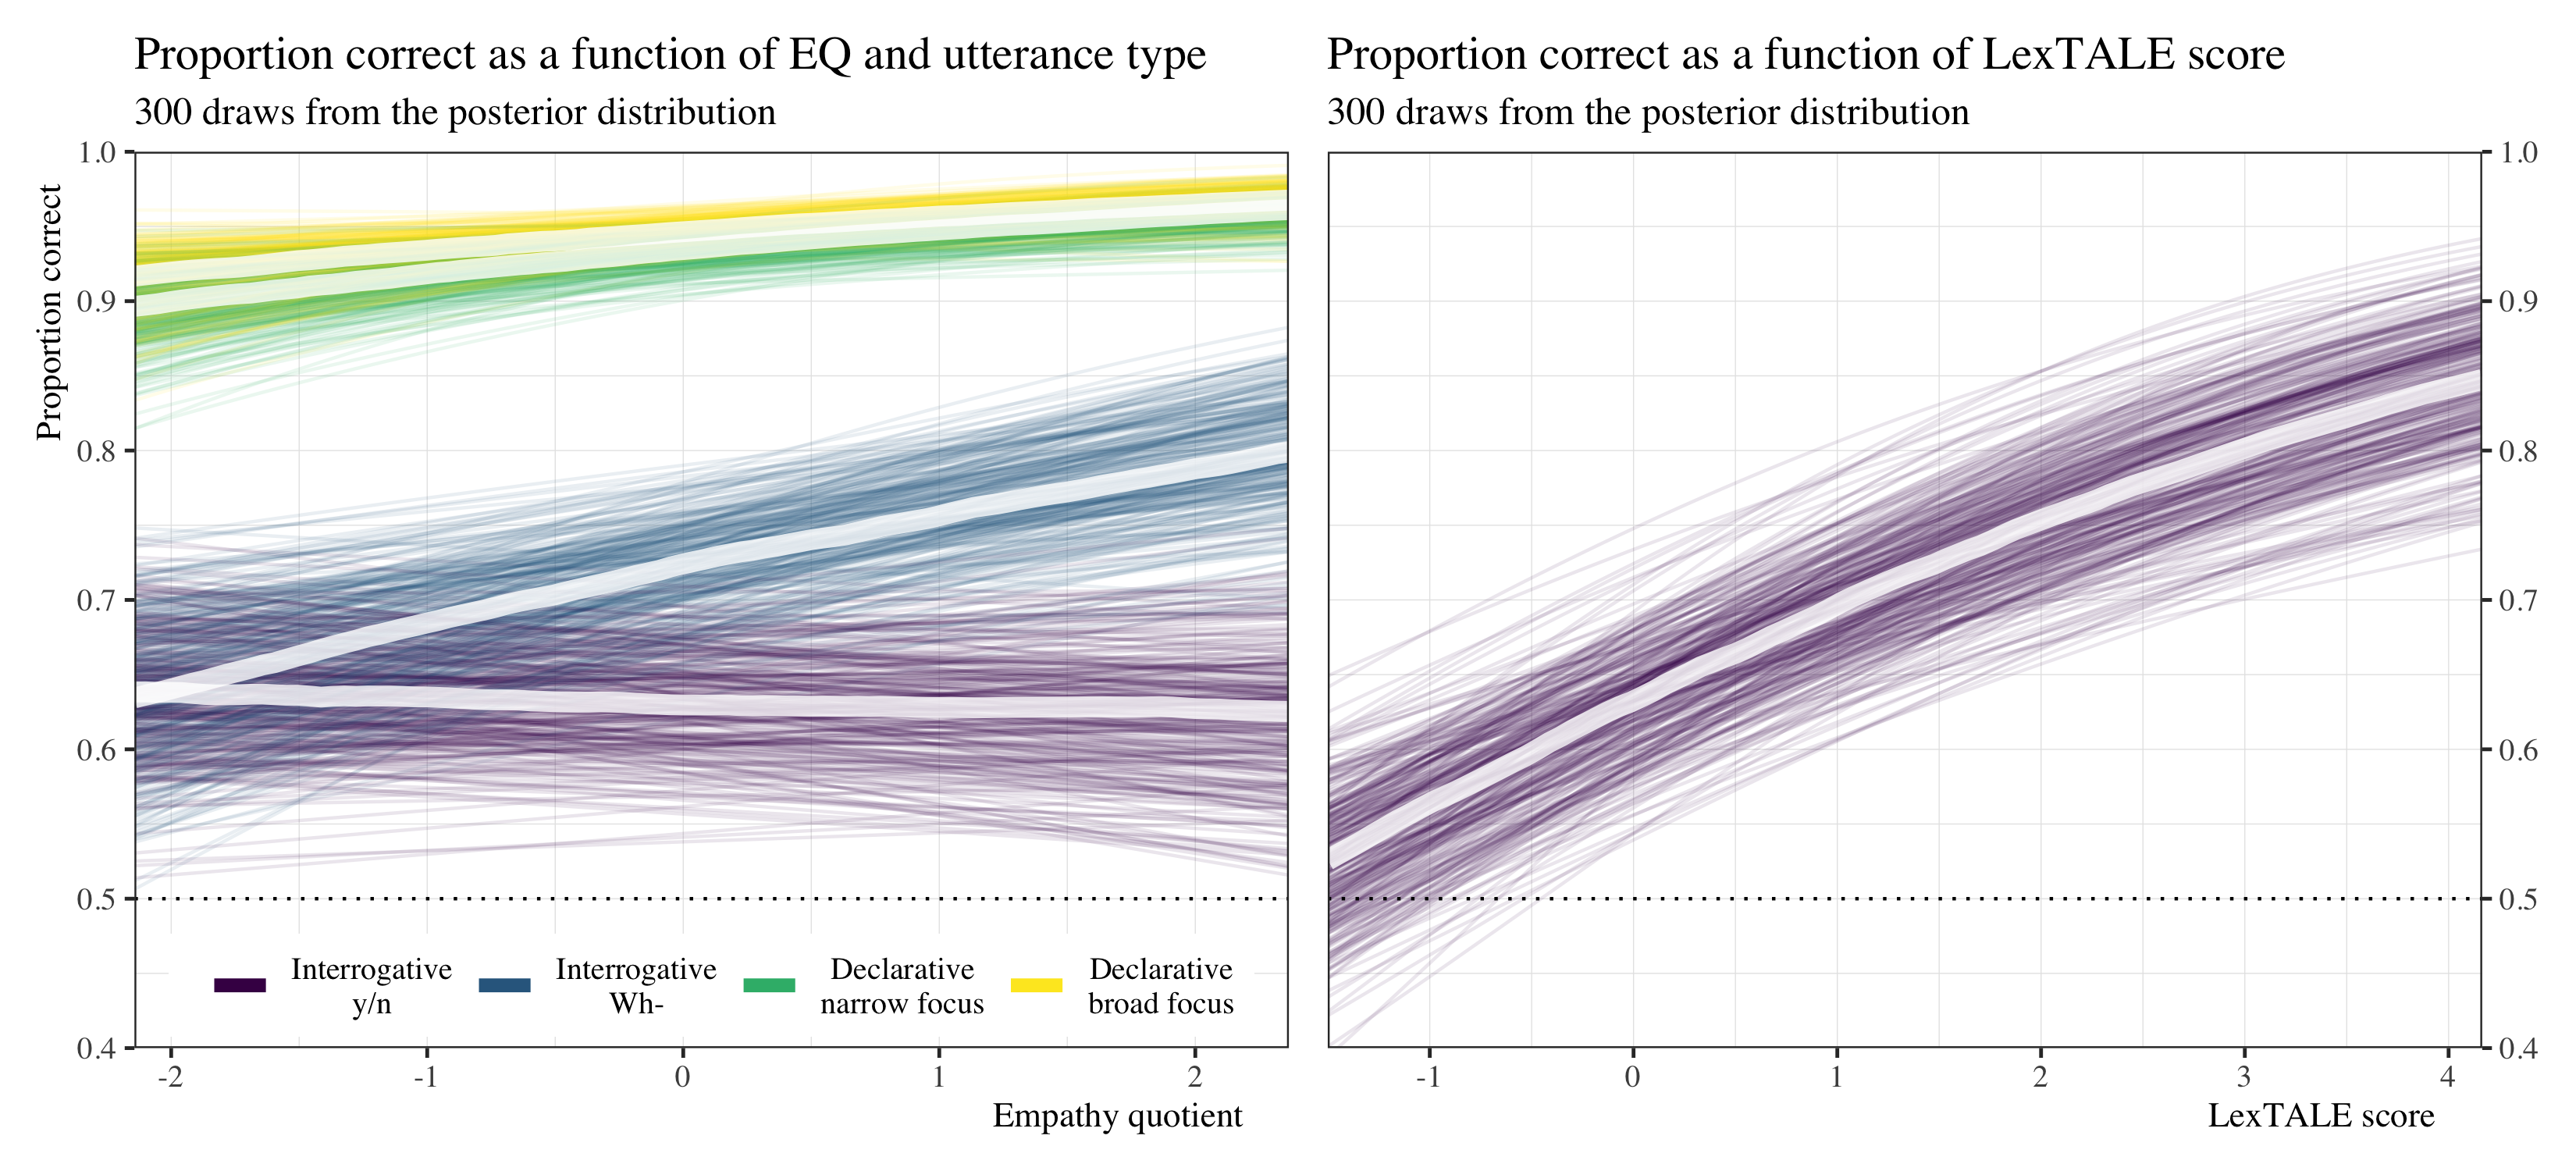
\includegraphics[width=1\linewidth]{/Users/casillas/academia/research/in_progress/empathy_intonation_perc/figs/abstract/plot_abstract_hls} \caption{Conditional effects of response accuracy as a function of Empathy 
quotient and utterance type (panel A) and standardized LexTALE score (panel B). 
Individual colored lines represent 300 draws from the posterior distribution. White lines indicate the median lines of best fit from the posterior.}\label{fig:plot-2panel-emp-prof}
\end{figure}

\hypertarget{references}{%
\section{References}\label{references}}

\begingroup
\setlength{\parindent}{-0.5in}
\setlength{\leftskip}{0.5in}

\phantom{.}

\textcolor{white}{\\} \vspace{-0.5in}

\hypertarget{refs}{}
\begin{CSLReferences}{1}{0}
\leavevmode\hypertarget{ref-baron2004empathy}{}%
Baron-Cohen, S., \& Wheelwright, S. (2004). The empathy quotient: An
investigation of adults with asperger syndrome or high functioning
autism, and normal sex differences. \emph{Journal of Autism and
Developmental Disorders}, \emph{34}(2), 163--175.

\leavevmode\hypertarget{ref-bustin_2020}{}%
Brandl, A., González, C., \& Bustin, A. (2020). The development of
intonation in L2 spanish: A perceptual study. In A. Morales-Front, M. J.
Ferreira, R. P. Leow, \& C. Sanz (Eds.), \emph{Hispanic linguistics:
Current issues and new directions} (pp. 12--31). John Benjamins
Publishing Company.

\leavevmode\hypertarget{ref-esteve2020empathy}{}%
Esteve-Gibert, N., Schafer, A. J., Hemforth, B., Portes, C., Pozniak,
C., \& D'Imperio, M. (2020). Empathy influences how listeners interpret
intonation and meaning when words are ambiguous. \emph{Memory \&
Cognition}, 1--15. \url{https://doi.org/10.3758/s13421-019-00990-w}

\leavevmode\hypertarget{ref-izura2014lextale}{}%
Izura, C., Cuetos, F., \& Brysbaert, M. (2014). Lextale-esp: A test to
rapidly and efficiently assess the spanish vocabulary size.
\emph{Psicol{ó}gica}, \emph{35}(1), 49--66.

\leavevmode\hypertarget{ref-trofimovich2006learning}{}%
Trofimovich, P., \& Baker, W. (2006). Learning second language
suprasegmentals: Effect of L2 experience on prosody and fluency
characteristics of L2 speech. \emph{Studies in Second Language
Acquisition}, 1--30. \url{https://doi.org/10.1017/S0272263106060013}

\end{CSLReferences}

\endgroup

\end{document}
